\section{Reddit Level Interactions}
As found in prior work, subreddits maintain particular levels of toxicity community norms~\cite{rajadesingan2020quick}. For example, as found by Rajadesingan \textit{et al.}, the subreddit WhiteRights had much higher tolerance for toxic content than the subreddits NeutralPolitics or AskEconomics. In this section, we analyze how distinctive political norms and toxicity levels within given subreddits contribute to levels of misinformation. 


In order to get an approximation of the levels of misinformation within a given subreddit we utilize a set of 157,605 \textit{misinformation-oriented} websites. We define \textit{misinformation-oriented} websites as websites that have more connections from our set of misinformation websites than from authentic news (i.e., the majority of a site's inward links in a domain-based graph are from misinformation websites. Websites that have been widely documented as spreading falsehood and conspiracy theories are included within this list including InfoWars and 8kun.top~\cite{hanley2022no,starbird2018ecosystem}.


As seen in Figure~\ref{figure:misinfo-toxciity-polarization}, there are political and toxicity norms across the spectrum, with polarization levels not being correlated levels of toxicity nor with misinformation levels. We see in particular that subreddits that are at the edge of political spectrum actually have some of the lowest average Perspective Toxicity scores and the lowest amounts of misinformation hyperlinks. We thus see at that at the edges of the political spectrum, where users are more isolated and insular that the overall levels of toxicity within the subreddit are not as high as those more ``moderate'' subreddits. This suggests that these cohesive communities where users are more similar to each other may producing the least amounts of bad behavioral outcomes. 


As seen in Figure~{}, toxicity the


\begin{figure}
\centering
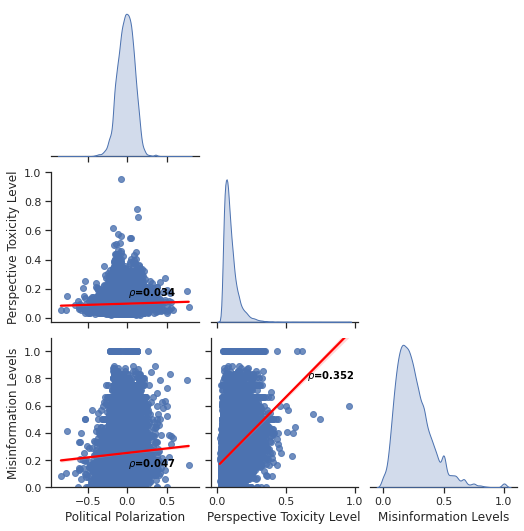
\includegraphics[width=0.75\columnwidth]{figures/subreddit_distribution.png} 
\caption{\textbf{Distributions of political polarization, perspective toxicity levels, and misinformation-oriented URL usage across subreddits with at least 100 users }--- While previous research has indicated that political polarization and toxicity are heavily correlated, we see in Reddit's case due to its self-selecting communities that political polarization is not correlated with vitriol and comment toxicity. Similarly we see that political polarization is not correlated with misinformation levels. Rather subreddits within the political center have the highest percentages of misinformation and toxicity. 
}
\label{figure:misinfo-toxciity-polarization}
\end{figure}